\documentclass[a4paper,12pt,oneside]{article}

\usepackage{geometry}
\geometry{a4paper,top=2cm,bottom=2cm,left=2cm,right=2cm,heightrounded,bindingoffset=5mm}

\usepackage[T1]{fontenc}
\usepackage[utf8]{inputenc}
\usepackage[english]{babel}
\usepackage{hyperref}
\usepackage{caption}
\usepackage{subfig}
\usepackage{graphicx}
\usepackage{amsmath}
\usepackage{mathtools}
\usepackage[dvipsnames]{xcolor}
\usepackage{fontspec}
\newfontfamily\ubuntumono[Scale=0.95]{Ubuntu Mono}
\definecolor{light}{gray}{0.4}

\usepackage{minted}

%abs and norm
\DeclarePairedDelimiter{\abs}{\lvert}{\rvert}
\DeclarePairedDelimiter{\norm}{\lVert}{\rVert}

%%%%%%%%%%%%%%%%%%%%%%%%%%%%%%%%%%%%%%%%%%%%%%%%%%

%to deal with indentation
\newlength\tindent
\setlength{\tindent}{\parindent}
\setlength{\parindent}{0pt}
\renewcommand{\indent}{\hspace*{\tindent}}

%\indent This is some text that will be indented.

%%%%%%%%%%%%%%%%%%%%%%%%%%%%%%%%%%%%%%%%%%%%%%%%%%

\begin{document}

\author{Eduardo Quintana \and Luca Bonaldo}
\title{Binary search tree - anlysis report}
\maketitle

This is a data analysis report of the performance of the binary search tree code written for the course of Advanced Programming, Master in HPC, SISSA. 

\section{Scope}
The scope of this analysis is to check that the lookup of the implemented binary search tree scales logaritmically with respect to the number of nodes.

\section{Procedure}
In order to study the performances of the lookup of the implemented binary seach tree, an \textbf{analysis.cpp} code has been written. This code is structured as follows:

\begin{itemize}
\item Four types of tree are studied (the first argument is the type of the \textbf{\textcolor{blue}{key}}, the second of the \textbf{\textcolor{blue}{value}}):
  \begin{enumerate}
  \item \begin{minted}[style=vi]{cpp}
      map<int,double>
    \end{minted}
  \item \begin{minted}[style=vi]{cpp}
      map<double,double>;
    \end{minted}
  \item \begin{minted}[style=vi]{cpp}
      map<string,double>;
    \end{minted}
  \item \begin{minted}[style=vi]{cpp}
      map<string,string>.
    \end{minted}
  \end{enumerate}
\item the tree is filled and checked using random number and string generators;
\item performances are deduced from the time taken by the implemented \textbf{find} function of the tree class on retriving a decided number of values;
\item the lookup time is taken firsly from the \textbf{unbalanced} tree and then from the \textbf{balanced} one. Both lookups are compared to the performances of the \textbf{std::map} provided by the C++ STD library;
\item the time is collected using the library \textbf{std::chrono}. 
\end{itemize}

The code has been run on Ulysses with the following parameters:
\begin{itemize}
\item tree-dimensions: 5000, 10000, 15000, 20000, 30000, 50000, 100000, 150000, 200000, 300000, 500000, 800000, 1000000 and 2000000 nodes;
\item number of lookups: 50, 100, 200, 500, 1000, 2000, 3000 and 50000 keys.
\end{itemize}

For every case, a sample of ten measurements has been taken in order to use the average as the most probable value with its associated standard error. From these data, several plots have been obtained, both in linear and log scale. All of them are collected in the \textit{analysis} folder.

\section{Results}
In the following plots some of the obtained results are reported according to different types of the tree and number of lookups.\\
The plots are reported in an increasing order in the number of lookups. For simplicity, just few of them have been shown, even if all of them can be found in the \textit{analysis} directory of the code. Moreover, for the \textbf{balanced} and \textbf{std::map} cases. the linear-scale case is compared with the log one in order to visualize and verify the logarithmic behaviuor of the find function of the tree.\\

\vspace{2.5cm}

% \begin{figure}
%   \begin{center}
%     \subfloat[][\emph{comparison plot}]{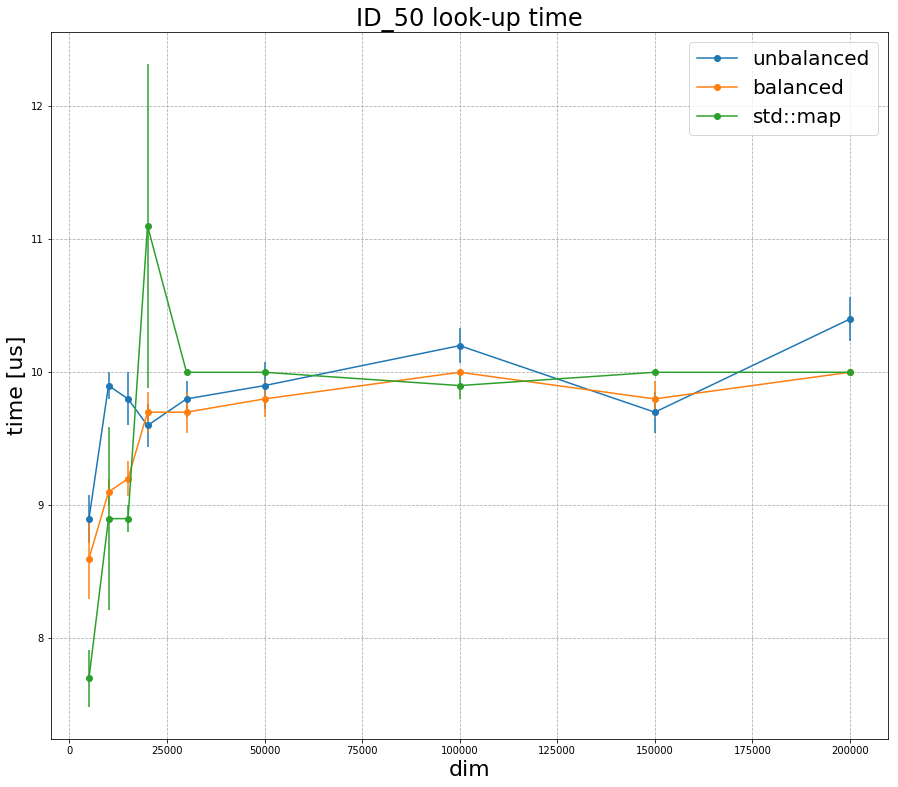
\includegraphics[width=0.5\textwidth]{ID_all_mean_50.png}}
%     \subfloat[][\emph{unbal linear scale}]{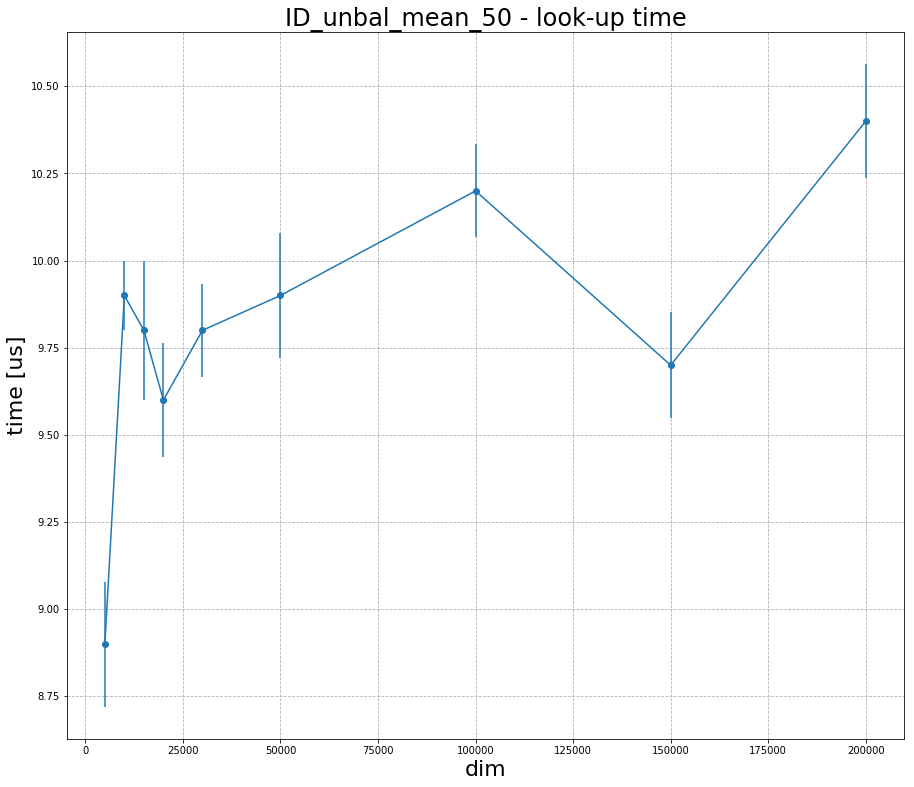
\includegraphics[width=0.5\textwidth]{ID_unbal_mean_50_lin.png}}\\
%     \subfloat[][\emph{bal linear scale}]{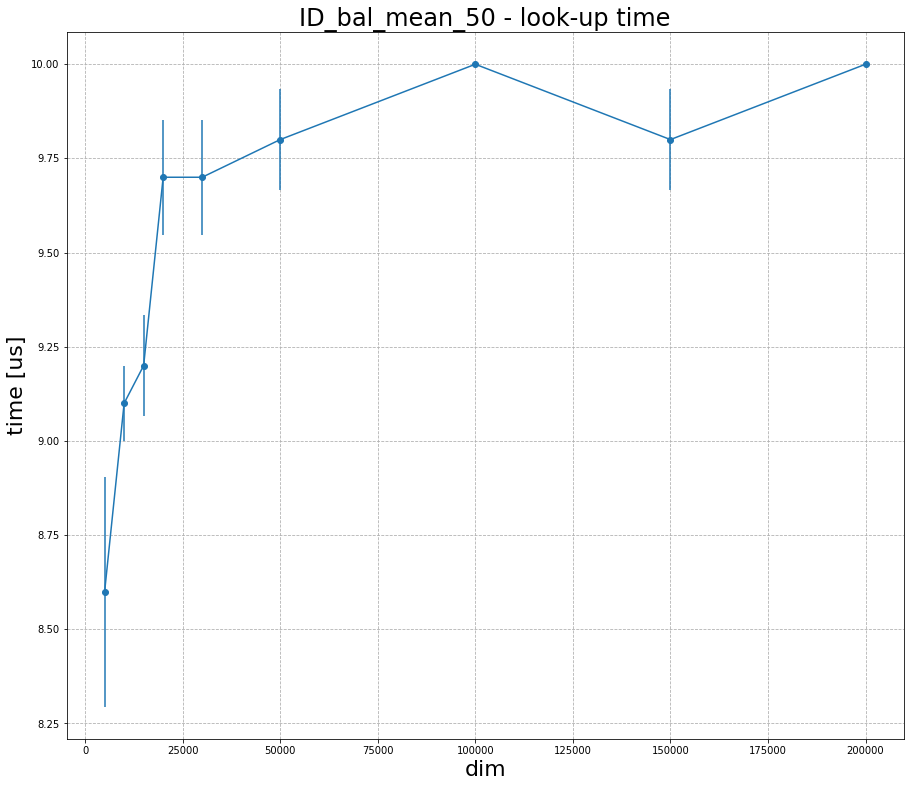
\includegraphics[width=0.5\textwidth]{ID_bal_mean_50_lin.png}}
%     \subfloat[][\emph{bal log scale}]{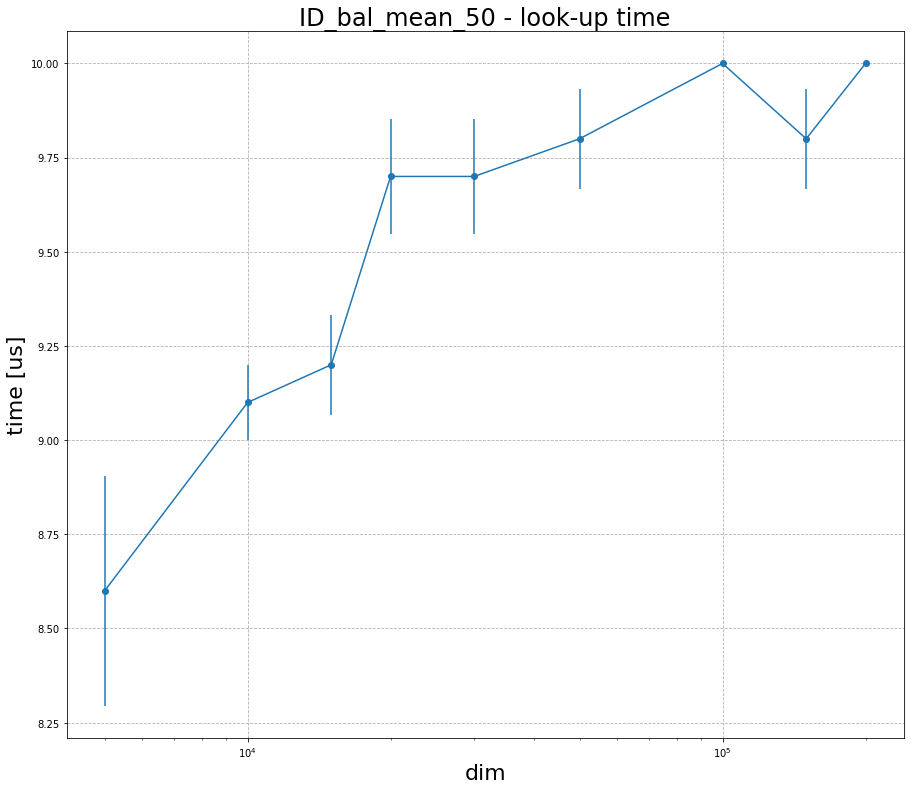
\includegraphics[width=0.5\textwidth]{ID_bal_mean_50_log.png}}
%   \end{center}
% \end{figure}

% \begin{figure}
%   \begin{center}
%     \subfloat[][\emph{std::map linear scale}]{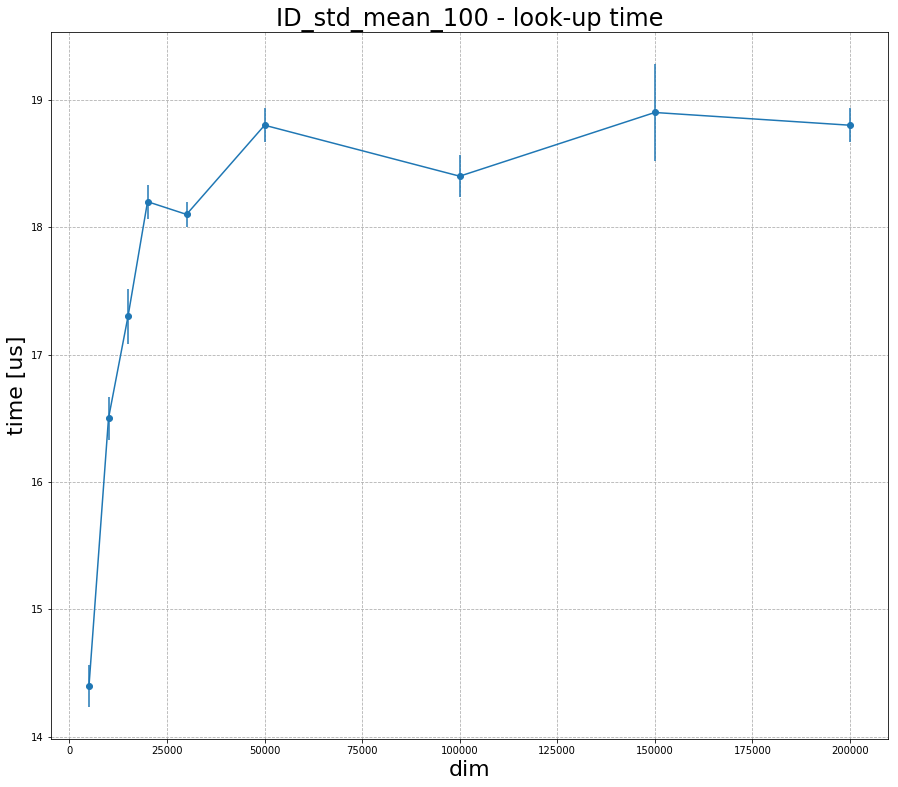
\includegraphics[width=0.5\textwidth]{ID_std_mean_100_lin.png}}
%     \subfloat[][\emph{std::map log scale}]{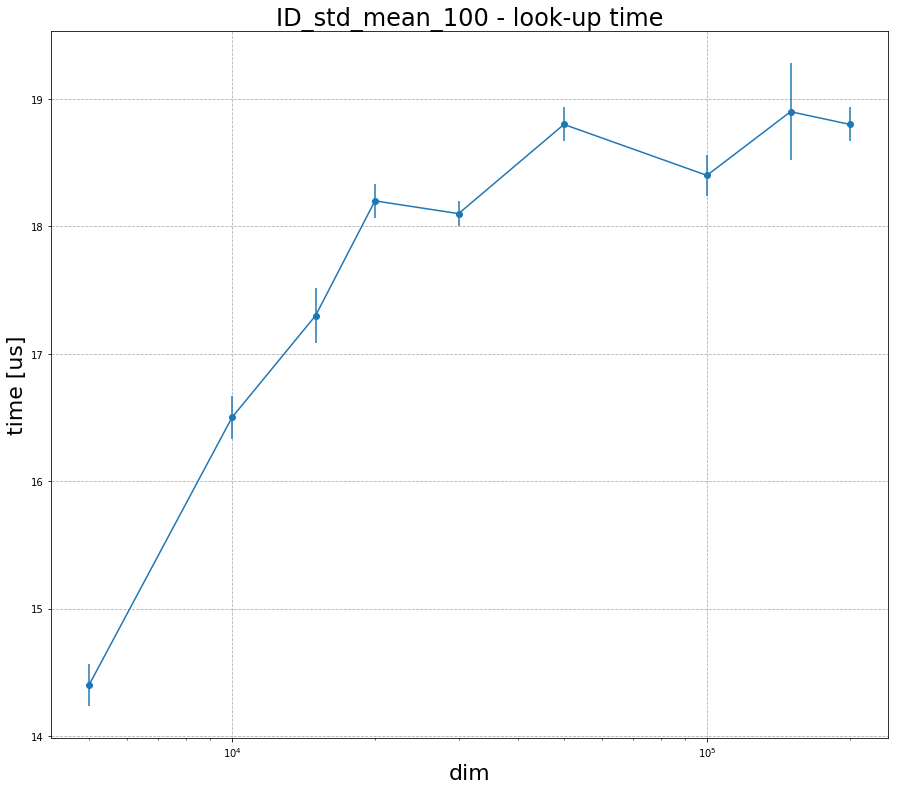
\includegraphics[width=0.5\textwidth]{ID_std_mean_100_log.png}}
%   \end{center}
% \end{figure}

\begin{figure}
  \begin{center}
    \subfloat[][\emph{linear scale}]{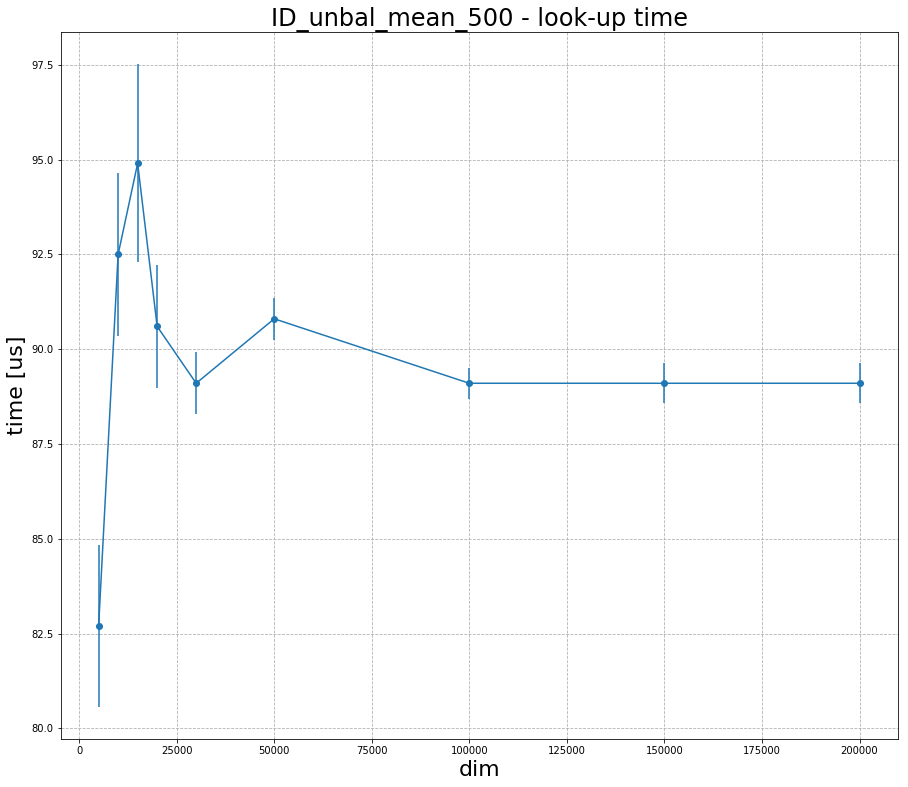
\includegraphics[width=0.5\textwidth]{ID_unbal_mean_500_lin.png}}
    \subfloat[][\emph{comparison plot}]{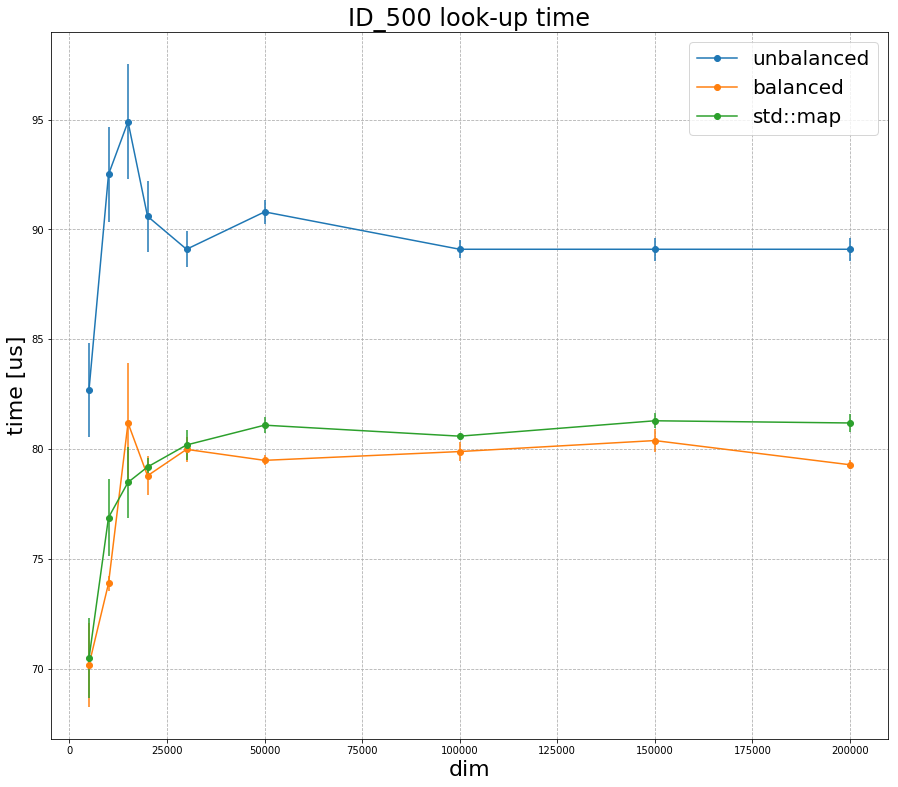
\includegraphics[width=0.5\textwidth]{ID_all_mean_500.png}}
  \end{center}
\end{figure}

\begin{figure}
  \begin{center}
    \subfloat[][\emph{linear scale}]{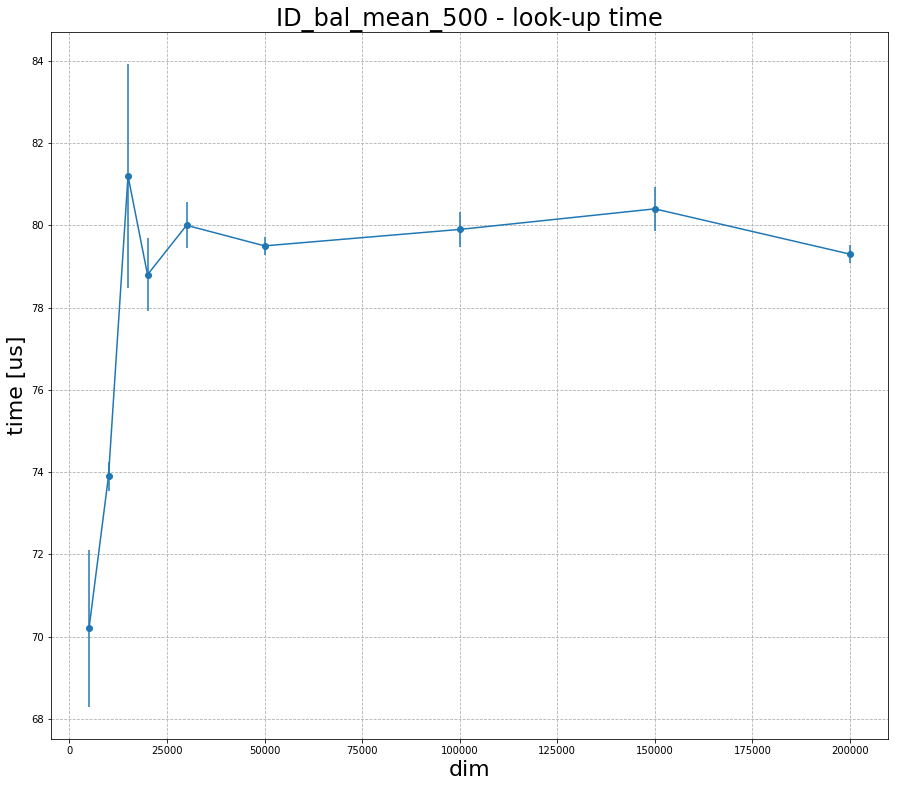
\includegraphics[width=0.5\textwidth]{ID_bal_mean_500_lin.png}}
    \subfloat[][\emph{log scale}]{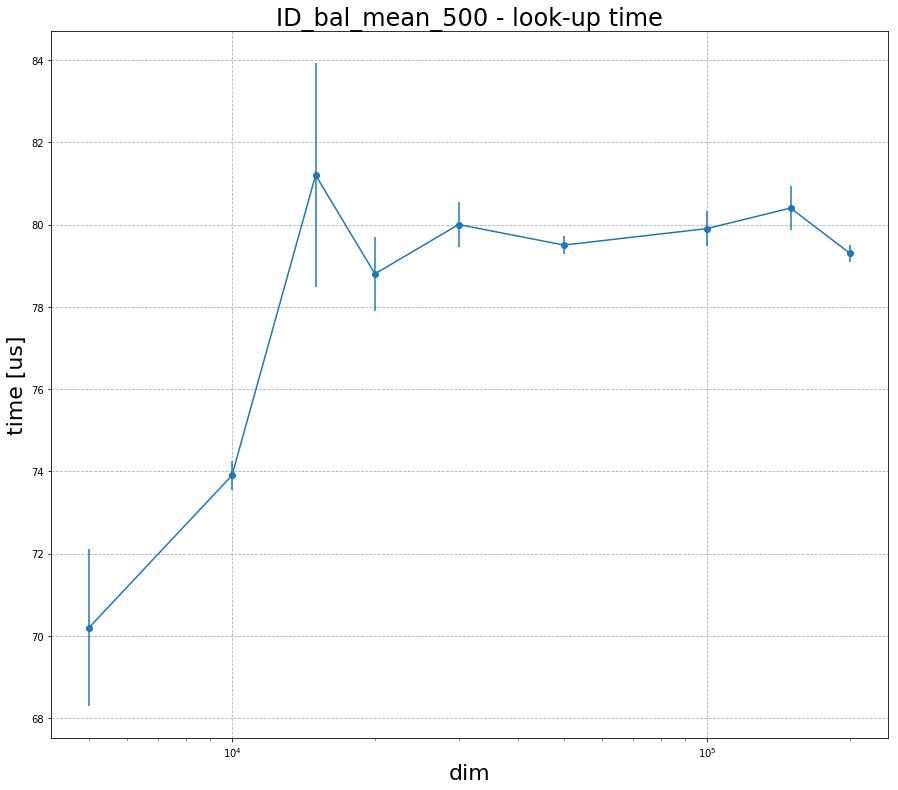
\includegraphics[width=0.5\textwidth]{ID_bal_mean_500_log.png}}
  \end{center}
\end{figure}

\begin{figure}
  \begin{center}
    \subfloat[][\emph{linear scale}]{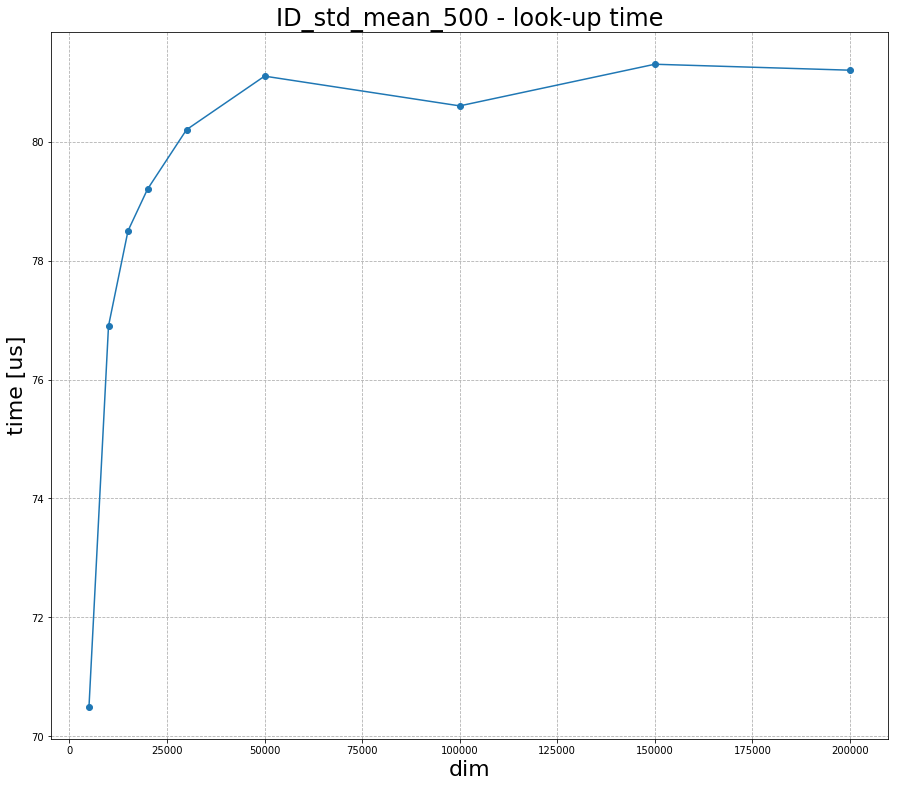
\includegraphics[width=0.5\textwidth]{ID_std_mean_500_lin.png}}
    \subfloat[][\emph{log scale}]{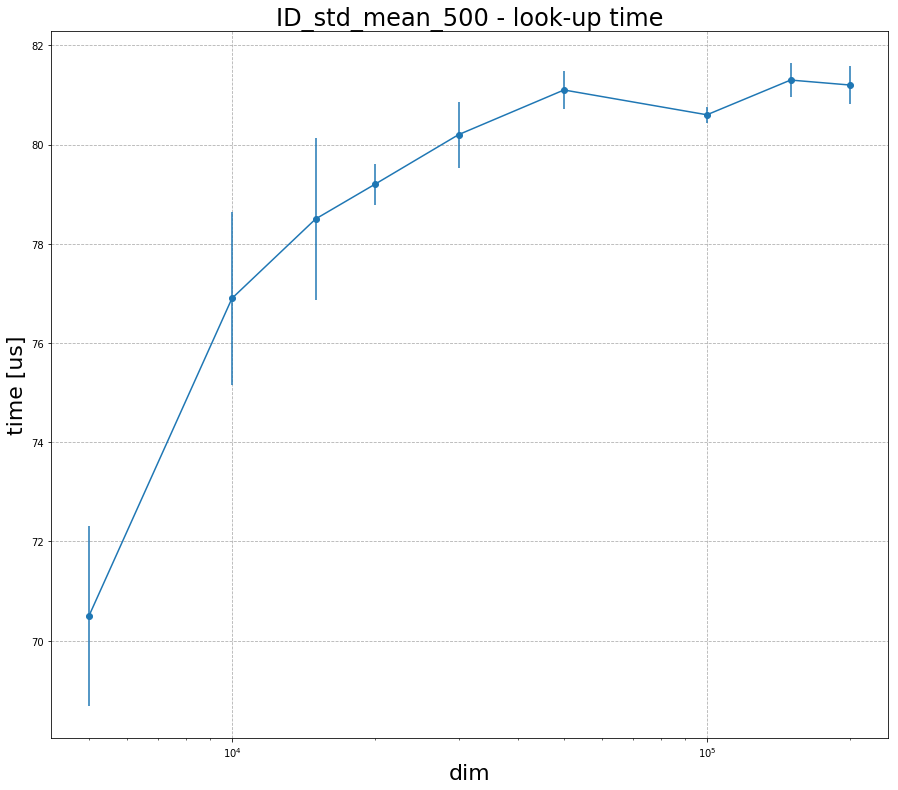
\includegraphics[width=0.5\textwidth]{ID_std_mean_500_log.png}}
  \end{center}
\end{figure}

As we can see from these plots, as we increase the number of lookup, the error bars shrink, the linear plots get closer to a logarithmic function as the log-scale plots approache a linear behaviour for big dimensions of the tree and large numbers of lookup. The plots are also reported with a rise in the complexity of the  tree (i.e. from integers and doubles to strings).\\

From these results we can infer that the find function of the implemented binary tree shows a good behaviuor with incresing dimension when compared to the one implemented in the $c++$ standard library, even if the performances are $7\% \sim  10\%$ lower. This fact was expected and seems reasonable, although a deeper profiling of the code could be done in order to better these performances. However, from these results, we can still conclude that the lookup of the binary tree that we implemented behaves as $O(\log{N})$ for big dimensions of the tree.\\

\begin{figure}
  \begin{center}
    \subfloat[]{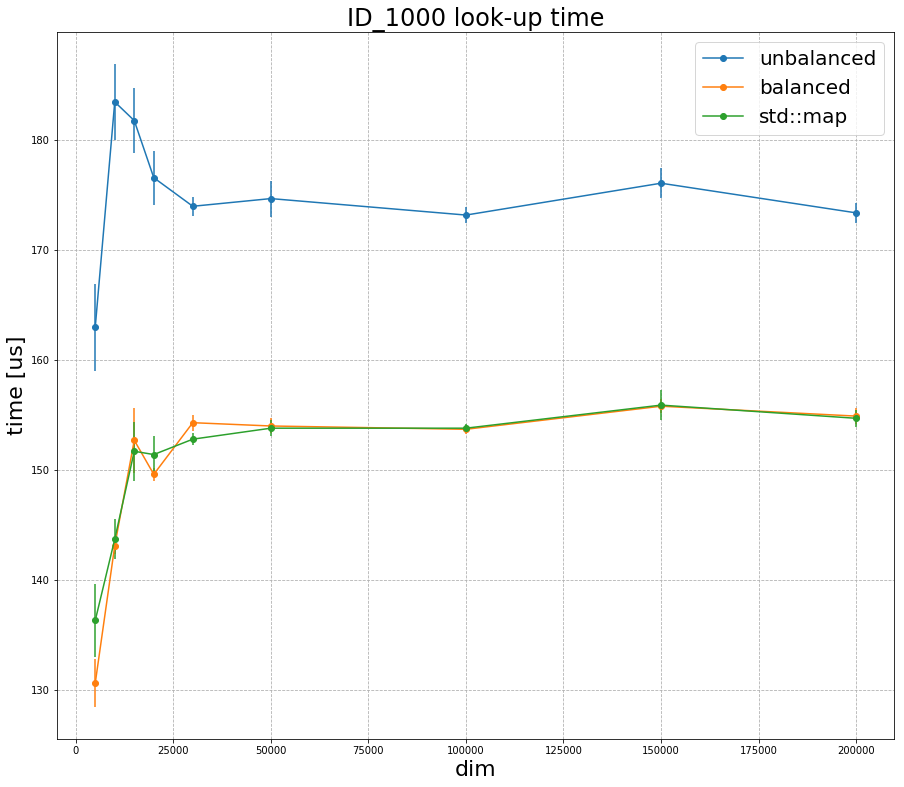
\includegraphics[width=0.5\textwidth]{ID_all_mean_1000.png}}
    \subfloat[]{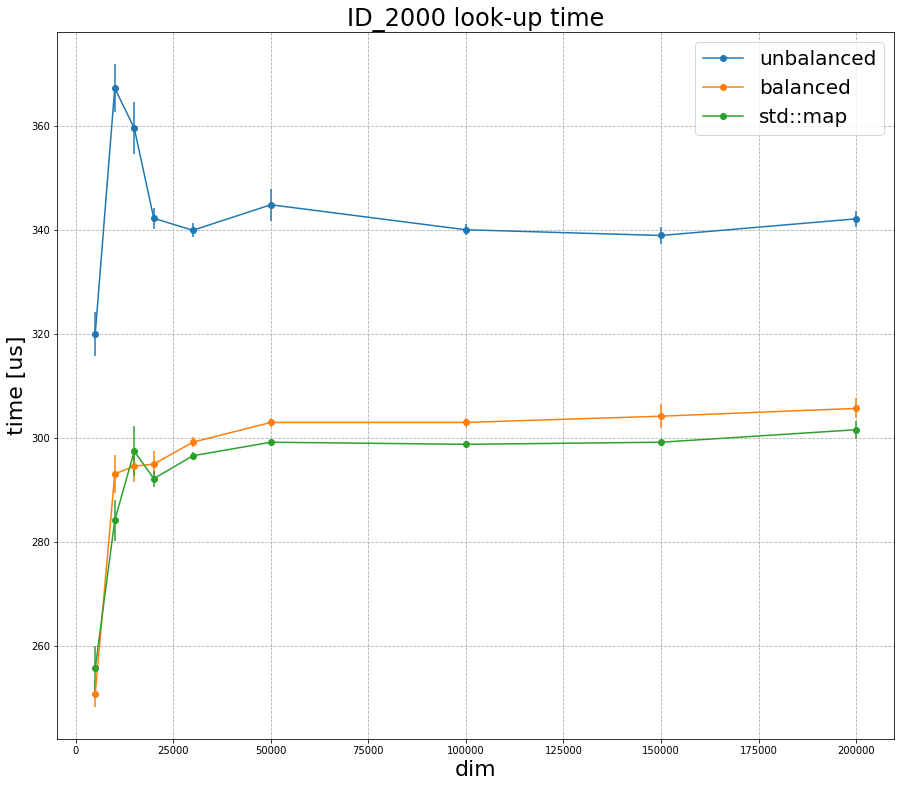
\includegraphics[width=0.5\textwidth]{ID_all_mean_2000.png}}
  \end{center}
\end{figure}

\begin{figure}
  \begin{center}
    \subfloat[][\emph{linear scale}]{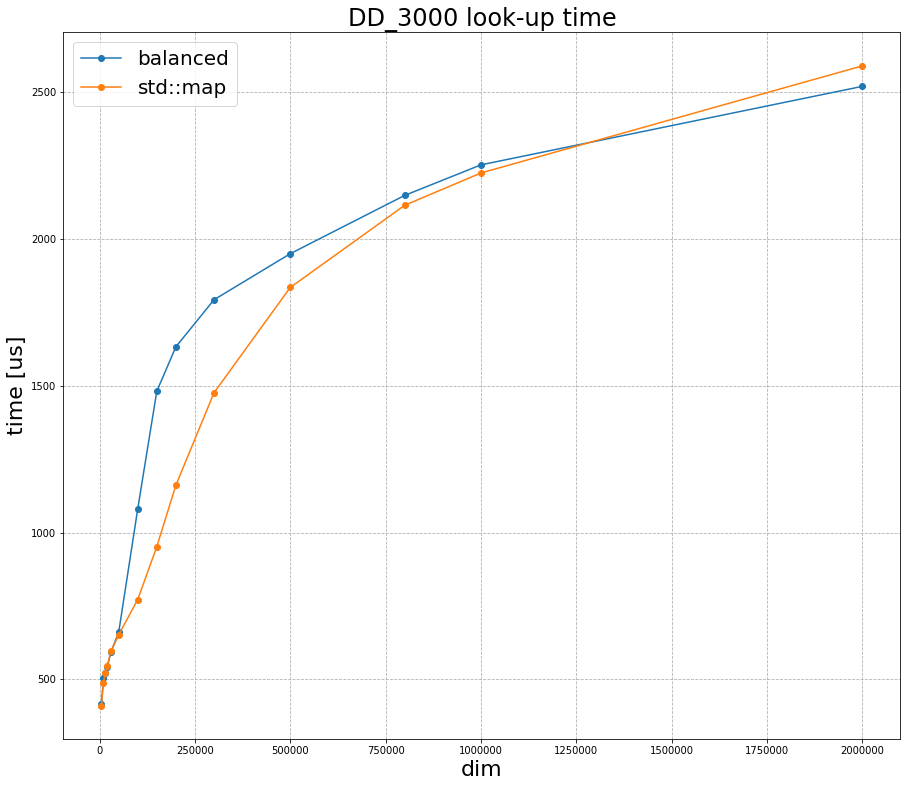
\includegraphics[width=0.5\textwidth]{DD_all_mean_3000.png}}
    \subfloat[][\emph{log scale}]{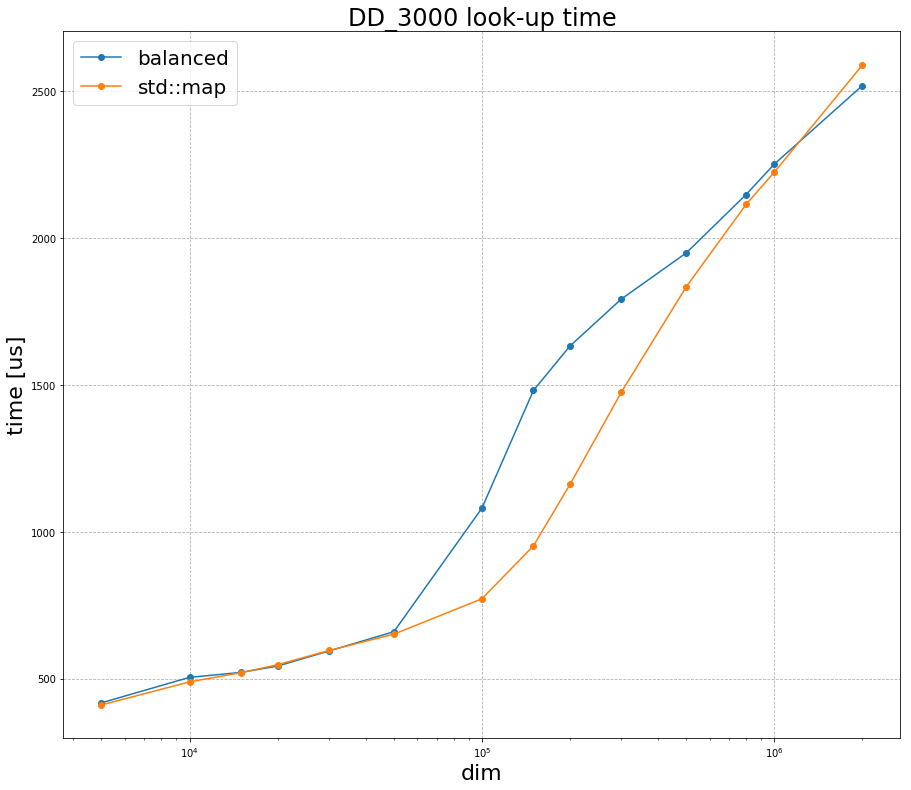
\includegraphics[width=0.5\textwidth]{DD_all_mean_3000_log.png}}\\
    \subfloat[][\emph{linear scale}]{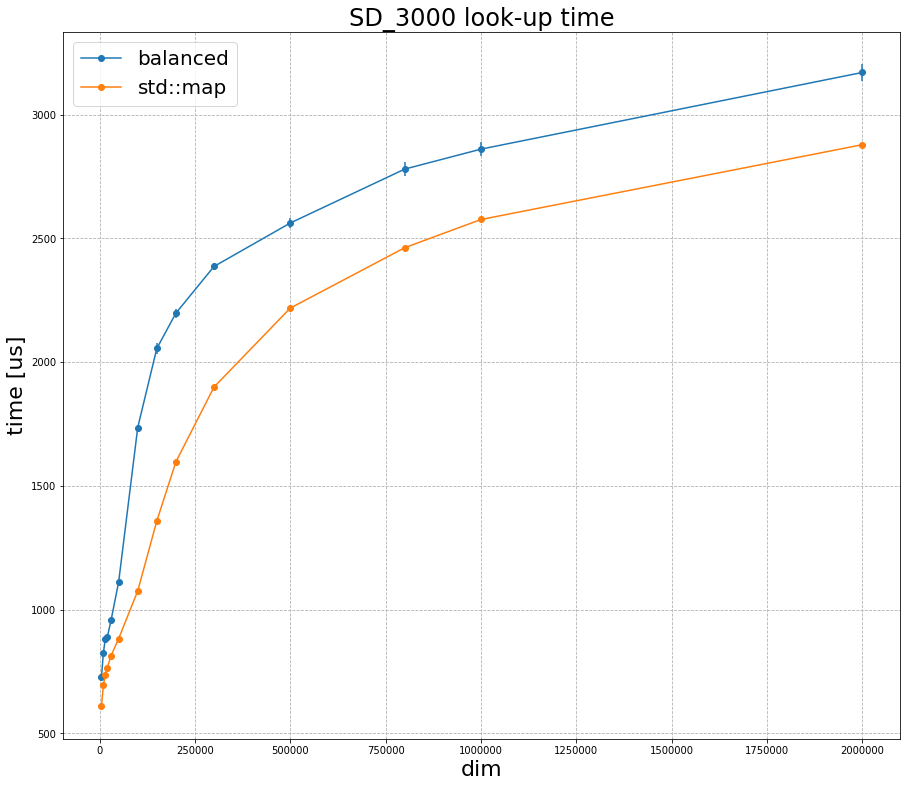
\includegraphics[width=0.5\textwidth]{SD_all_mean_3000.png}}
    \subfloat[][\emph{log scale}]{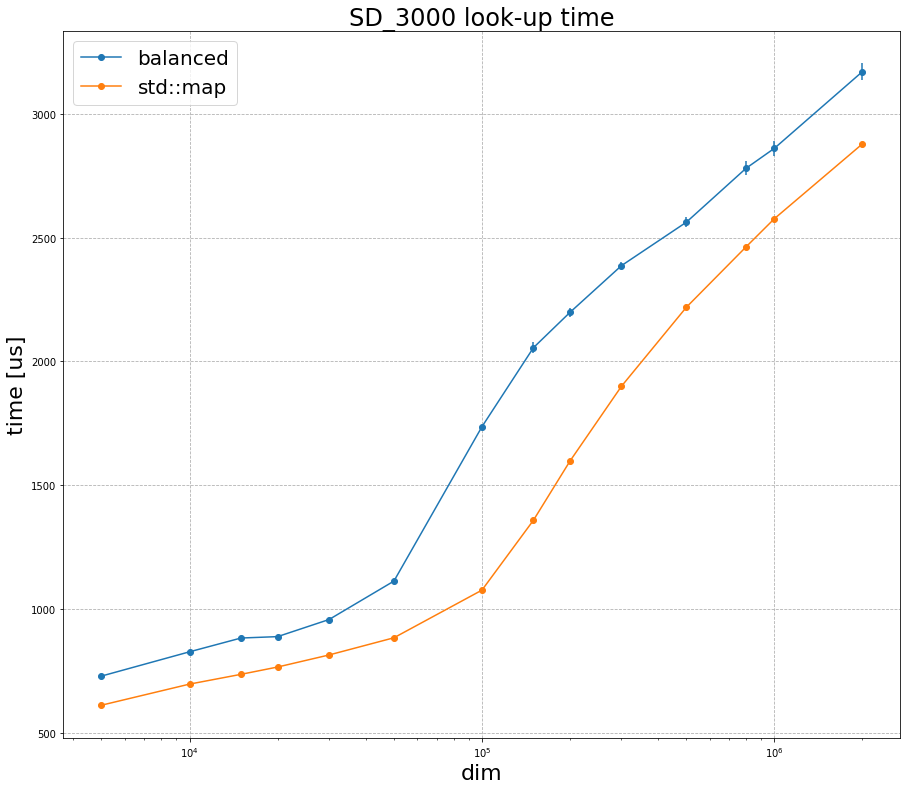
\includegraphics[width=0.5\textwidth]{SD_all_mean_3000_log.png}}\\
    \subfloat[][\emph{linear scale}]{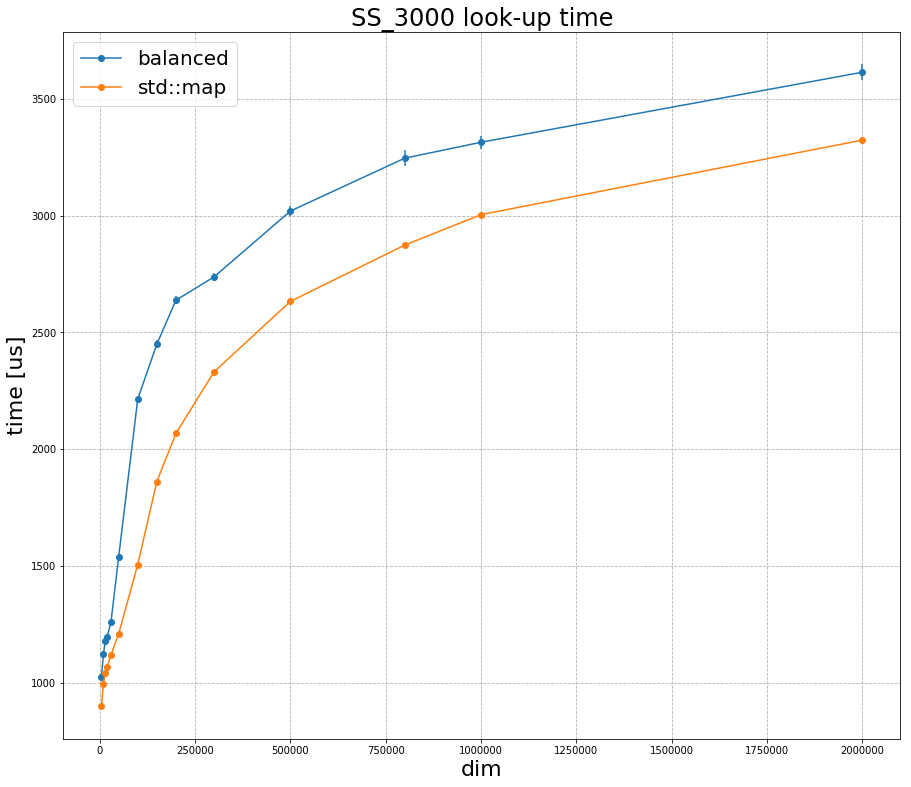
\includegraphics[width=0.5\textwidth]{SS_all_mean_3000.png}}
    \subfloat[][\emph{log scale}]{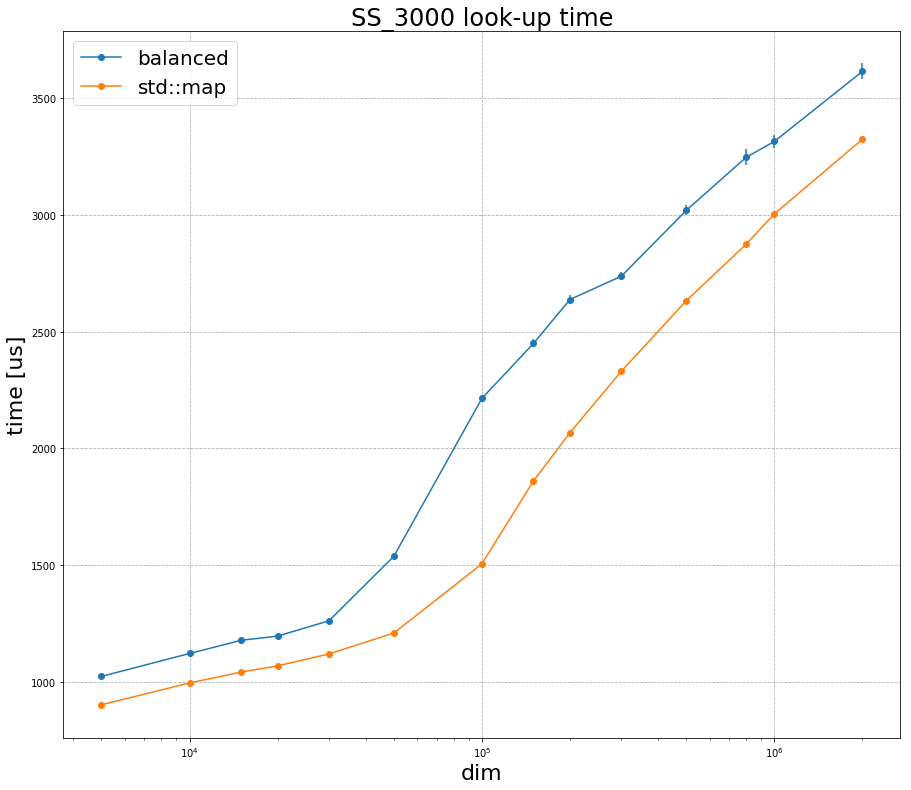
\includegraphics[width=0.5\textwidth]{SS_all_mean_3000_log.png}}
  \end{center}
\end{figure}

\begin{figure}
  \begin{center}
    \subfloat[][\emph{linear scale}]{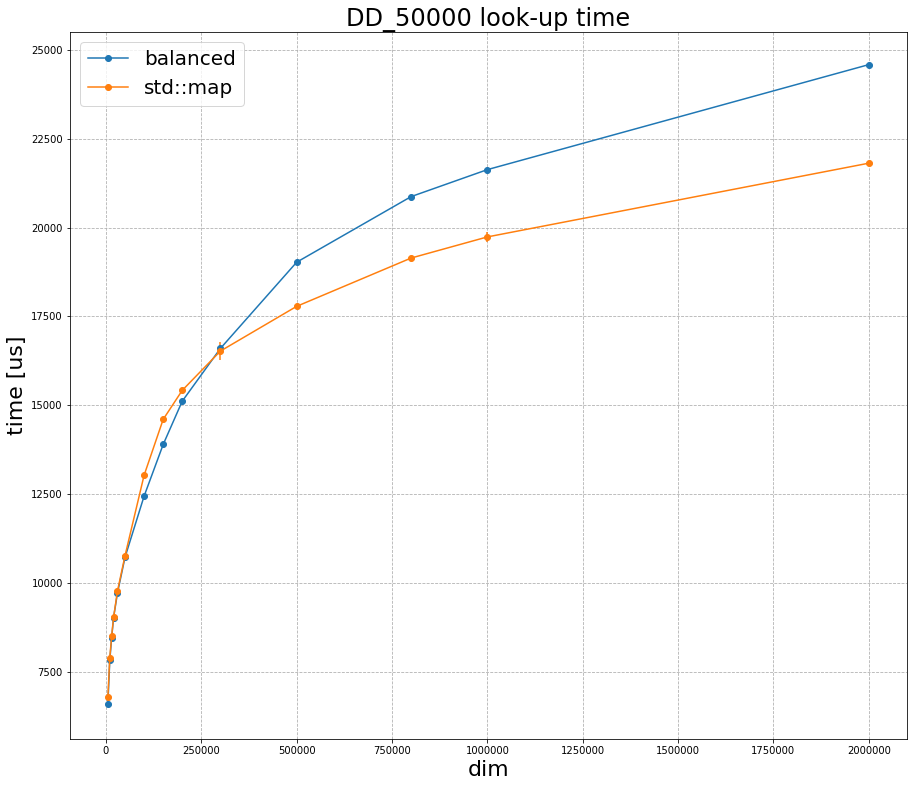
\includegraphics[width=0.5\textwidth]{DD_all_mean_50000.png}}
    \subfloat[][\emph{log scale}]{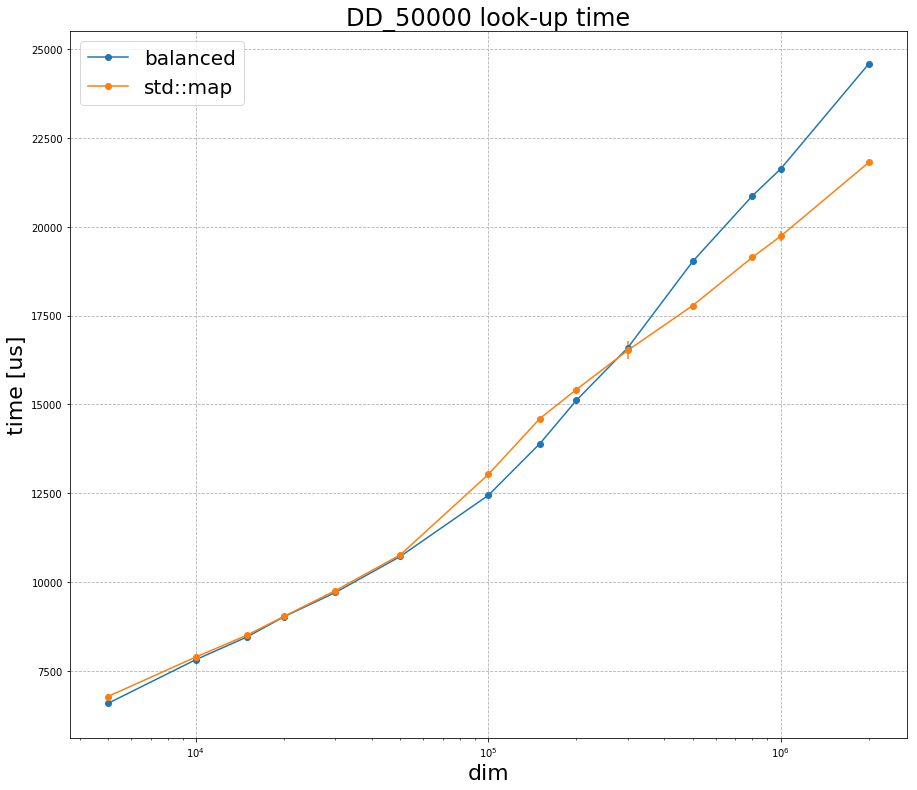
\includegraphics[width=0.5\textwidth]{DD_all_mean_50000_log.png}}\\    
    \subfloat[][\emph{linear scale}]{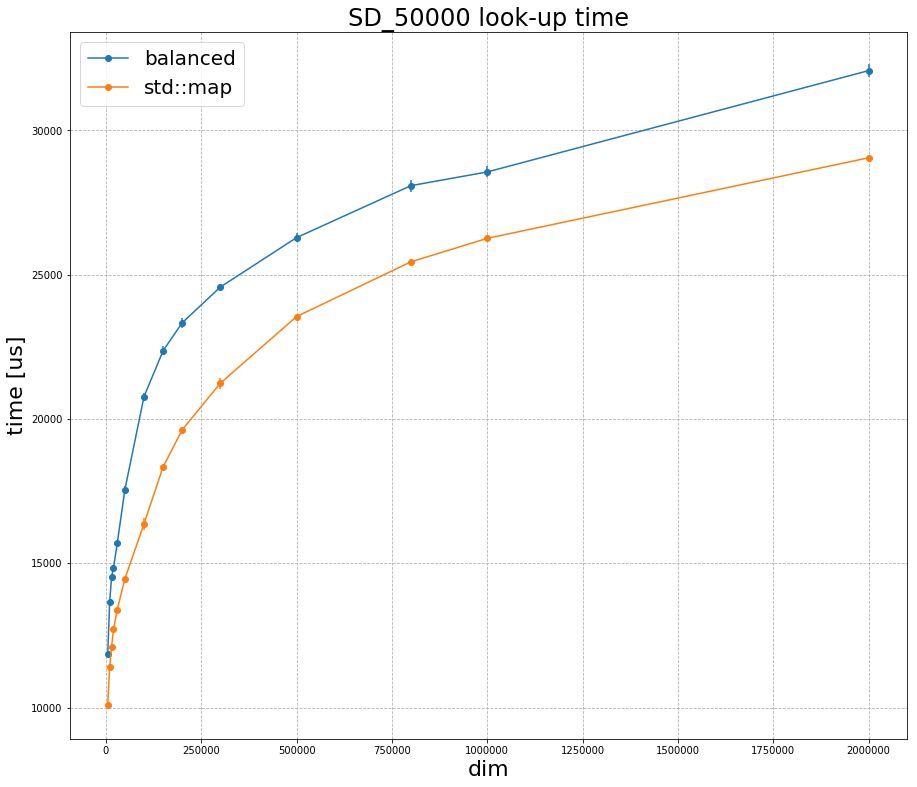
\includegraphics[width=0.5\textwidth]{SD_all_mean_50000.png}}
    \subfloat[][\emph{log scale}]{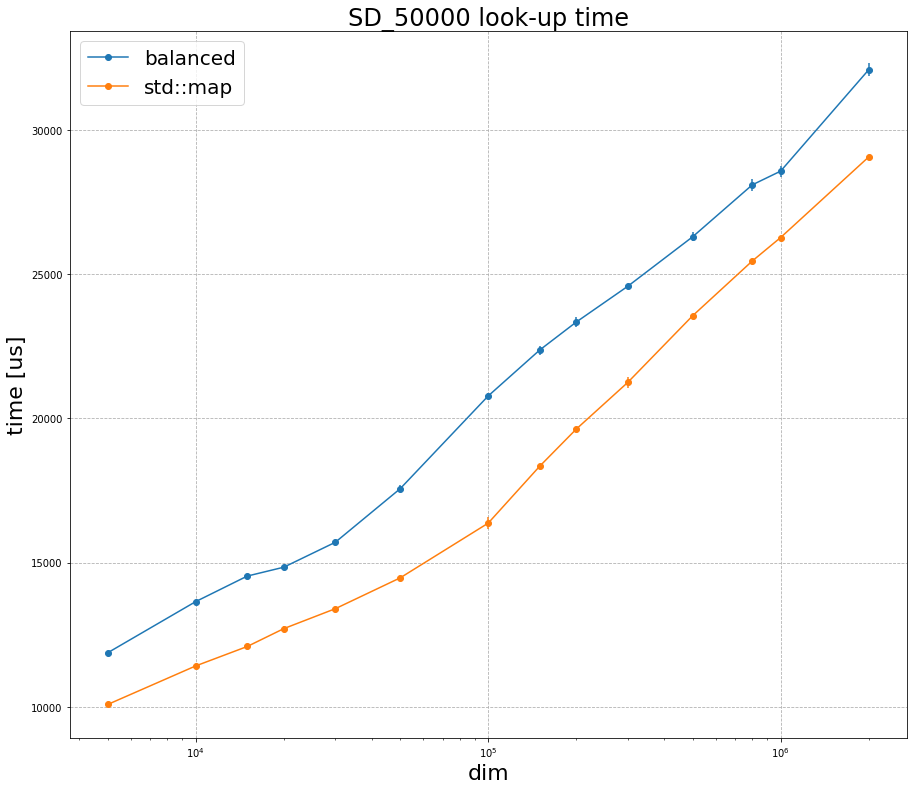
\includegraphics[width=0.5\textwidth]{SD_all_mean_50000_log.png}}\\
    \subfloat[][\emph{linear scale}]{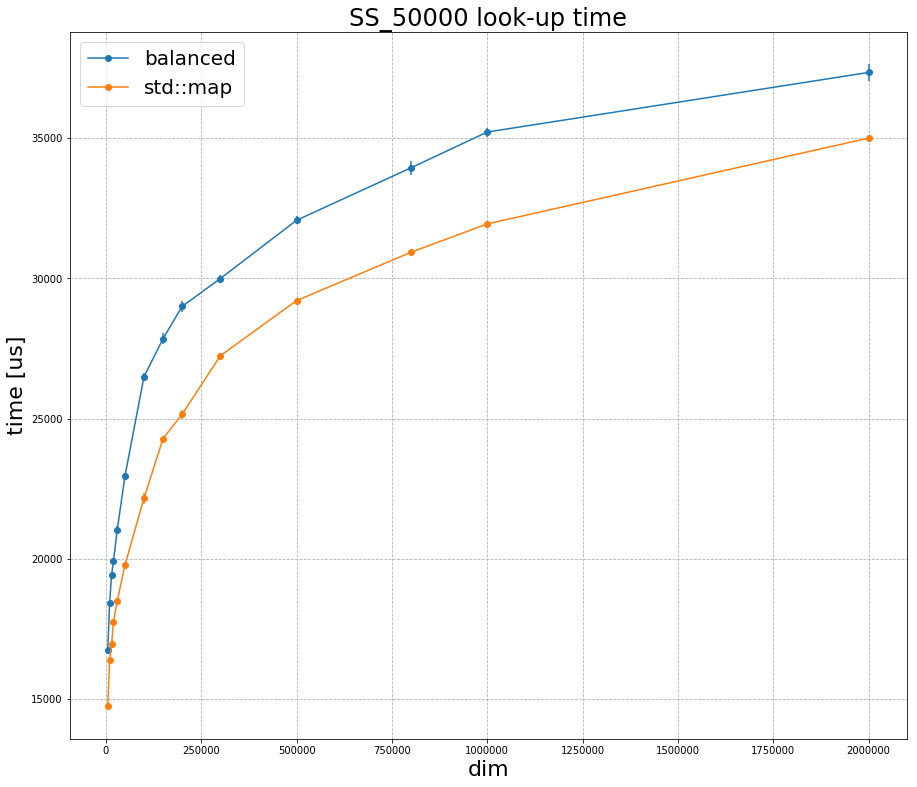
\includegraphics[width=0.5\textwidth]{SS_all_mean_50000.png}}
    \subfloat[][\emph{log scale}]{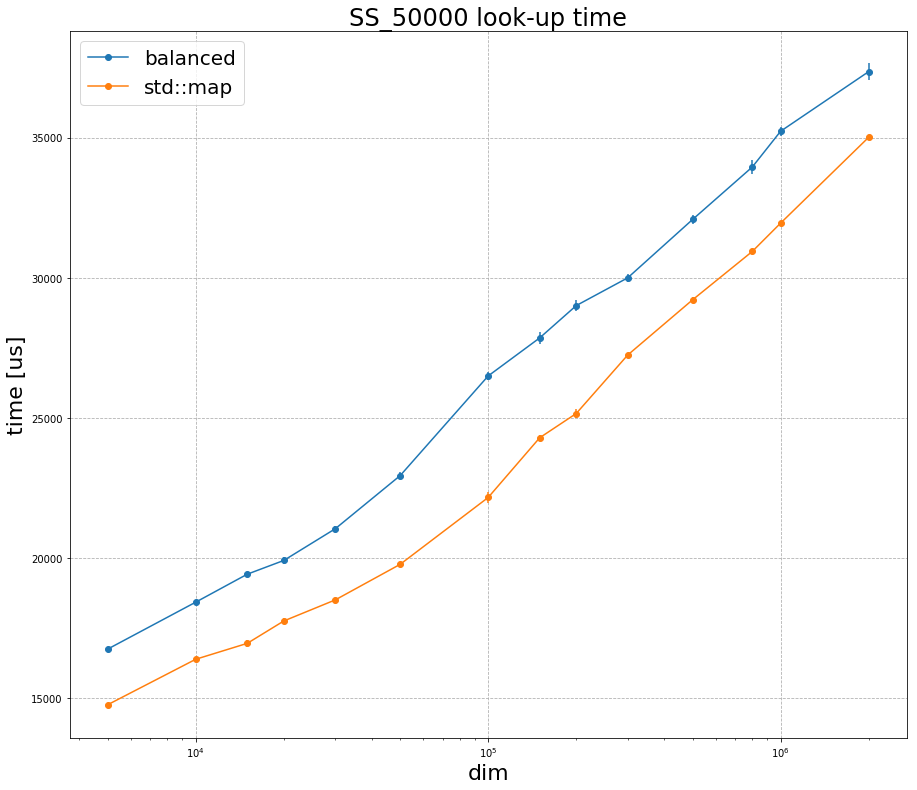
\includegraphics[width=0.5\textwidth]{SS_all_mean_50000_log.png}}\\
  \end{center}
\end{figure}

\end{document}
